%% dk 20190521 prostate page 1
%\documentclass{article}

\documentclass[border=5]{standalone}

\usepackage{tikz}
%\usepackage{xcolor}
\usetikzlibrary{arrows,shapes,snakes,automata,backgrounds,petri, decorations.text,positioning, calc}

\begin{document}
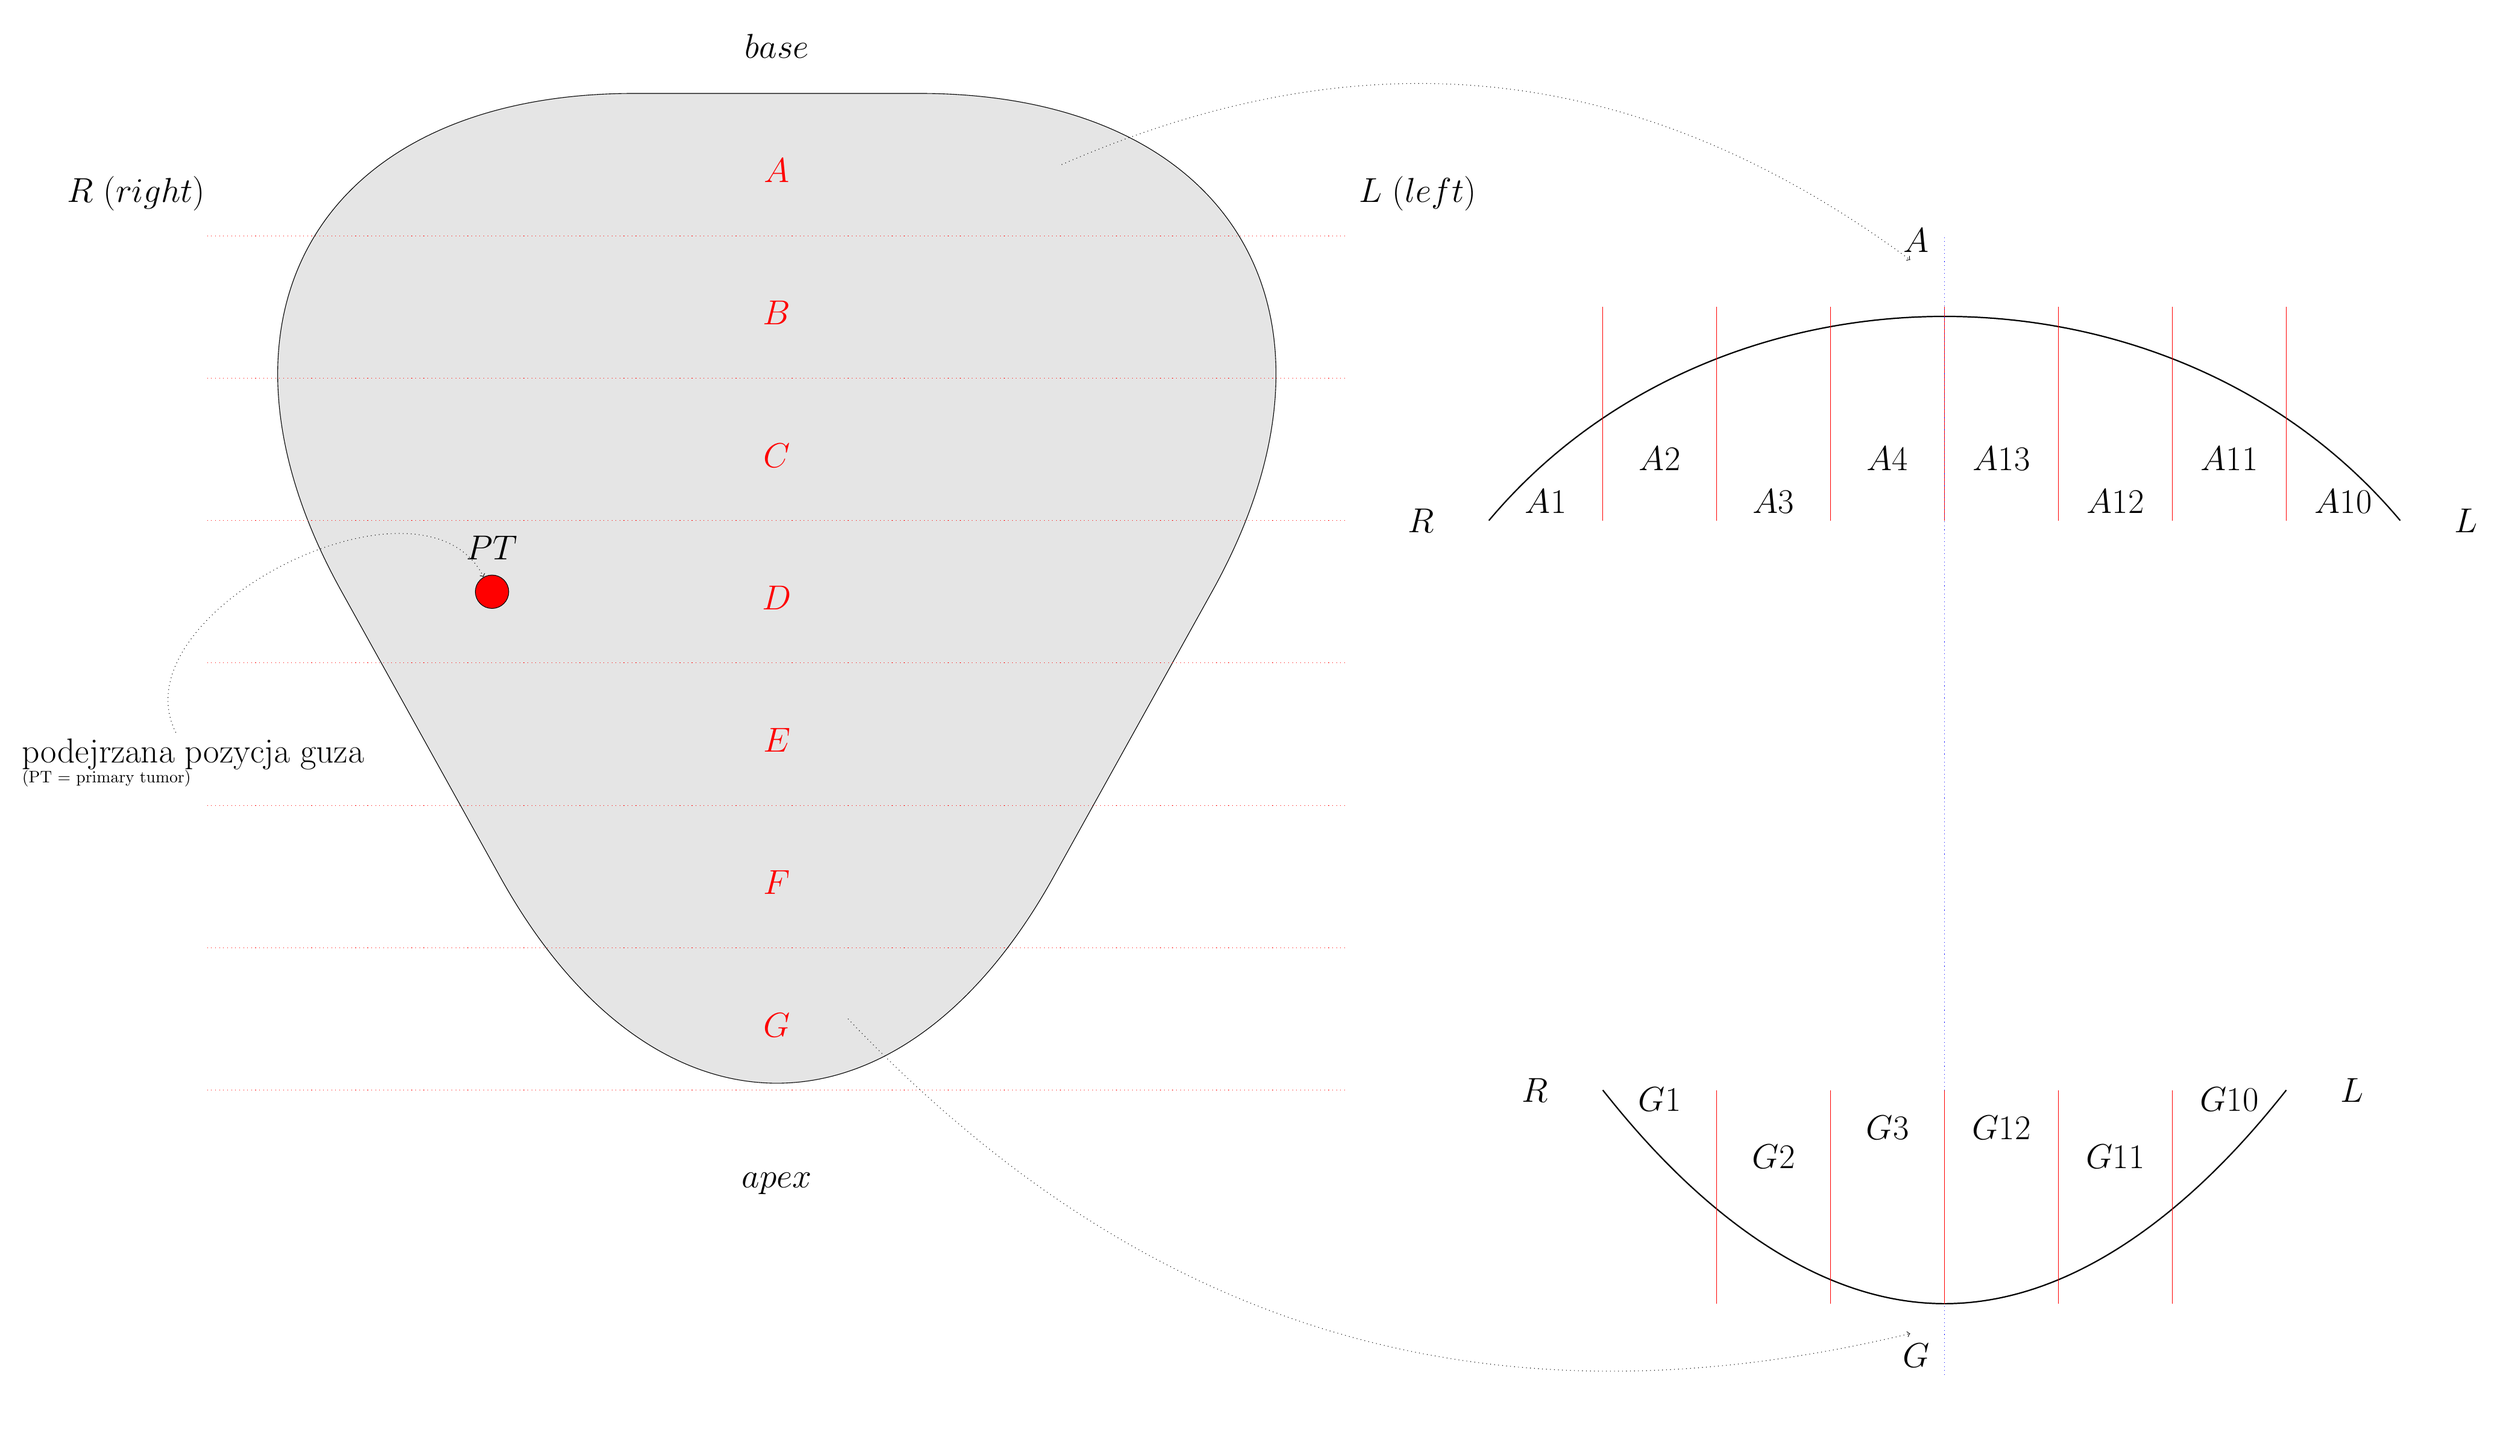
\begin{tikzpicture}[scale=3]
    \draw [rounded corners=120mm,fill=gray!20] (0,10)--(10,10)--(5,1)--cycle;
    
\draw[dotted, red] (  1,9)  -- node [above,  yshift=10mm] {\huge{$A$}} (9,9); 
\draw[dotted, red] (  1,8)  -- node [above,  yshift=10mm] {\huge{$B$}} (9,8); 
\draw[dotted, red] (  1,7)  -- node [above,  yshift=10mm] {\huge{$C$}} (9,7); 
\draw[dotted, red] (  1,6)  -- node [above,  yshift=10mm] {\huge{$D$}} (9,6); 
\draw[dotted, red] (  1,5)  -- node [above,  yshift=10mm] {\huge{$E$}} (9,5); 

 \draw[dotted, red] (  1,4)  -- node [above,  yshift=10mm] {\huge{$F$}} (9,4);
  \draw[dotted, red] (  1,3)  -- node [above,  yshift=10mm] {\huge{$G$}} (9,3);
 %label={[label distance=2mm]
  \node [circle,draw=black,fill=red,inner sep=0pt,minimum size=20pt,label={[label distance=2mm] {\huge{$PT$}}} ] (PT1) at (3,6.5) {};
  \node (box1) at  (0.9,5.3) [align=left] {\huge podejrzana pozycja guza\\(PT = primary tumor)} ;
 \draw[dotted, ->]
    (box1) [bend left=90]  to  (PT1);
 
 
  
\node [label=below:{\huge{$R\ (right) $}} ] (L) at (0.5,9.5) {};
\node [label=below:{\huge{$L\ (left) $}} ] (R) at (9.5,9.5) {};
\node [label=below:{\huge{$base$}} ] (base) at (5,10.5) {};
\node [label=below:{\huge{$apex$}} ] (apex) at (5,2.5) {};

\coordinate (A1_arc) at (10,7);
\coordinate (A2_arc) at (16.4,7);
\draw[thick] (A1_arc) [bend left=50]  to  (A2_arc);

\node [label=above:{\huge{$A$}} ] (A) at (13.0,8.8) {};

 \draw[dotted, ->]
    (7,9.5) [bend left=30]  to  (A);

\node [label=left:{\huge{$R$}} ] (A_R) at ($(A1_arc) - (0.3,0)$) {};

\node [label=right:{\huge{$L$}} ] (A_L) at ($(A2_arc) + (0.3,0)$) {};


\node [label=below:{\huge{$A1$}} ] (A1) at ($(A1_arc) + (0.4,0.3)$) {};

\draw[red]  ($(A1_arc) + (0.8,0)$) --  ($(A1_arc) + (0.8,1.5)$);

\node [label=below:{\huge{$A2$}} ] (A2) at ($(A1_arc) + (1.2,0.6)$) {};

\draw[red]  ($(A1_arc) + (1.6,0)$) --  ($(A1_arc) + (1.6,1.5)$);

\node [label=below:{\huge{$A3$}} ] (A3) at ($(A1_arc) + (2.0,0.3)$) {};

\draw[red]  ($(A1_arc) + (2.4,0)$) --  ($(A1_arc) + (2.4,1.5)$);

\node [label=below:{\huge{$A4$}} ] (A4) at ($(A1_arc) + (2.8,0.6)$) {};

\draw[red]  ($(A1_arc) + (3.2,0)$) --  ($(A1_arc) + (3.2,1.5)$);

\node [label=below:{\huge{$A13$}} ] (A14) at ($(A1_arc) + (3.6,0.6)$) {};

\draw[red]  ($(A1_arc) + (4,0)$) --  ($(A1_arc) + (4,1.5)$);

\node [label=below:{\huge{$A12$}} ] (A13) at ($(A1_arc) + (4.4,0.3)$) {};

\draw[red]  ($(A1_arc) + (4.8,0)$) --  ($(A1_arc) + (4.8,1.5)$);

\node [label=below:{\huge{$A11$}} ] (A12) at ($(A1_arc) + (5.2,0.6)$) {};

\draw[red]  ($(A1_arc) + (5.6,0)$) --  ($(A1_arc) + (5.6,1.5)$);

\node [label=below:{\huge{$A10$}} ] (A11) at ($(A1_arc) + (6,0.3)$) {};

\draw[blue, dotted]  (13.2, 1.0) -- (13.2, 9.0); 


\coordinate (G1_arc) at (10.8,3);
\coordinate (G2_arc) at (15.6,3);
\coordinate (G_arc_bottom) at (13.2, 1.5);
\draw[thick] (G_arc_bottom) parabola  (G1_arc);
\draw[thick] (G_arc_bottom) parabola  (G2_arc);

\node [label=below:{\huge{$G$}} ] (G) at ($(G_arc_bottom)-(0.2,0.2) $){};

\node [label=left:{\huge{$R$}} ] (G_R) at ($(G1_arc) - (0.3,0)$) {};

\node [label=right:{\huge{$L$}} ] (G_L) at ($(G2_arc) + (0.3,0)$) {};

\node [label=below:{\huge{$G1$}} ] (G1) at ($(G1_arc) + (0.4,0.1)$) {};

\draw[red]  ($(G1_arc) + (0.8,0)$) --  ($(G1_arc) + (0.8,-1.5)$);
 
\node [label=below:{\huge{$G2$}} ] (G2) at ($(G1_arc) + (1.2,-0.3)$) {};

\draw[red]  ($(G1_arc) + (1.6,0)$) --  ($(G1_arc) + (1.6,-1.5)$);

\node [label=below:{\huge{$G3$}} ] (G3) at ($(G1_arc) + (2.0,-0.1)$) {};

\draw[red]  ($(G1_arc) + (2.4,0)$) --  ($(G1_arc) + (2.4,-1.5)$);

\node [label=below:{\huge{$G12$}} ] (G13) at ($(G1_arc) + (2.8,-0.1)$) {};

\draw[red]  ($(G1_arc) + (3.2,0)$) --  ($(G1_arc) + (3.2,-1.5)$);

\node [label=below:{\huge{$G11$}} ] (G12) at ($(G1_arc) + (3.6,-0.3)$) {};

\draw[red]  ($(G1_arc) + (4.0,0)$) --  ($(G1_arc) + (4.0,-1.5)$);

\node [label=below:{\huge{$G10$}} ] (G11) at ($(G1_arc) + (4.4,0.1)$) {};
 
 \draw[dotted, ->]
    (5.5, 3.5) [bend right=30]  to  (G); 
 
% \node  (G) at (5,3.5) { G  } ;
 
%\draw[loosely  dotted] (-1,-1) grid (18,12);
\end{tikzpicture}
\end{document}